\subsection{Sprint 11: da 2024-08-05 a 2024-08-18}
\par Durante lo \glossario{sprint} 11, il team si impegna a completare la progettazione architetturale del \glossario{back-end} e la progettazione di dettaglio del \glossario{front-end}. Questo include la selezione definitiva del modello architetturale per il back-end. Inoltre, il gruppo prevede di compiere significativi progressi nella codifica del front-end. Infine, sono previste come attività la progettazione di dettaglio del back-end e la configurazione dell'ambiente di test.

\subsubsection{Obiettivi}
\begin{itemize}
  \item Stesura verbali interni;
  \item Stesura consuntivo \glossario{sprint} 10;
  \item Proseguimento progettazione logica \glossario{back-end} (definizione ad alto livello dei componenti, o route);
  \item Scelta definitiva del modello architetturale per il back-end;
  \item Stesura della sezione relativa allo stile architetturale nel documento di \ST;
  \item Inizio progettazione di dettaglio back-end;
  \item Separazione delle responsabilità del modulo index manager;
  \item Modifica dei tipi di ritorno del metodo di generazione del \glossario{prompt};
  \item Avanzamento codifica back-end;
  \item Ultimazione della progettazione di dettaglio \glossario{front-end};
  \item Definizione di tipi e interfacce con \glossario{TypeScript};
  \item Gestione centralizzata degli errori a front-end;
  \item Gestione messaggi di \glossario{debug} a front-end;
  \item Avanzamento codifica e testing front-end;
  \item Stesura del \MU\ nelle seguenti sezioni:
  \begin{itemize}
    \item Visualizzazione mobile;
    \item Sequenza di attività da svolgere per ottenere una query \glossario{SQL};
    \item Sezione di debug per il profilo Tecnico.
  \end{itemize}
  \item Ampliamento delle sezioni del \MU\ redatte nello sprint precedente;
  \item Configurazione di \glossario{SonarCloud} e integrazione con \glossario{GitHub};
  \item Individuazione di ulteriori strumenti per il controllo della qualità del codice;
  \item Aggiornamento della documentazione:
  \begin{itemize}
    \item \Gls;
    \item \NdP;
    \item \PdQ;
    \item \AdR;
    \item \ST.
  \end{itemize}
\end{itemize}

\begin{figure}[H]
  \centering
  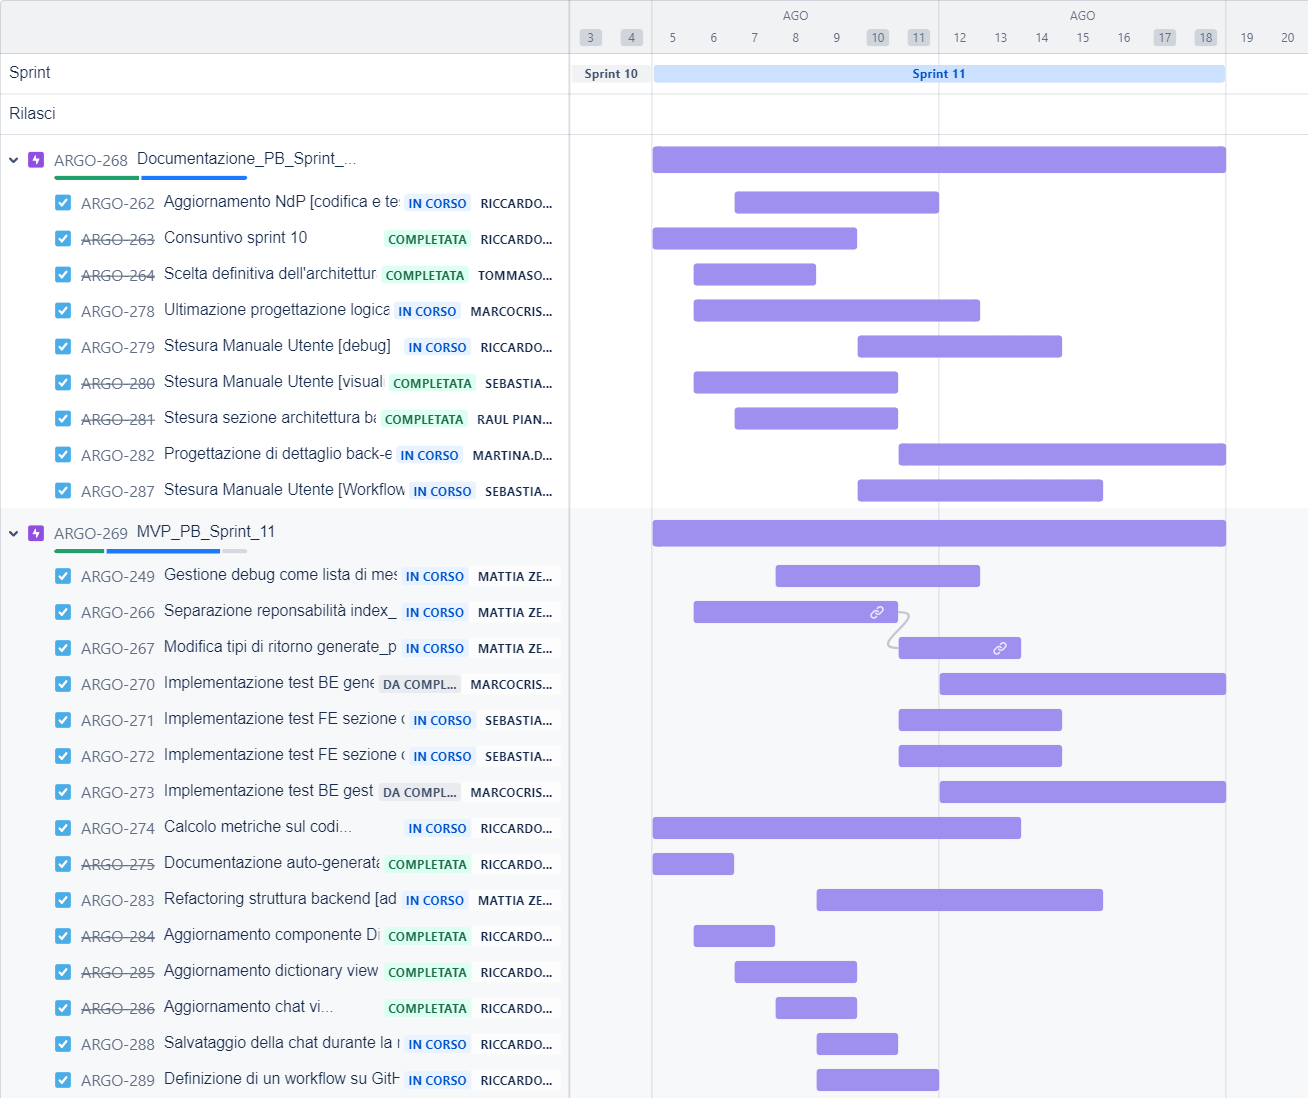
\includegraphics[width=0.90\textwidth]{assets/Pianificazione/Sprint-11/gantt.png}
  \caption{Sprint 11 - Diagramma di Gantt}\label{fig:sprint-10-gantt}
\end{figure}

